\centering
\begin{subfigure}[t]{0.48\textwidth}
  \centering
  % Test-pie source image is squarer than the spec-pie source (3-entry legend
  % vs. 5-entry); scaling down so the actual pie diameters match.
  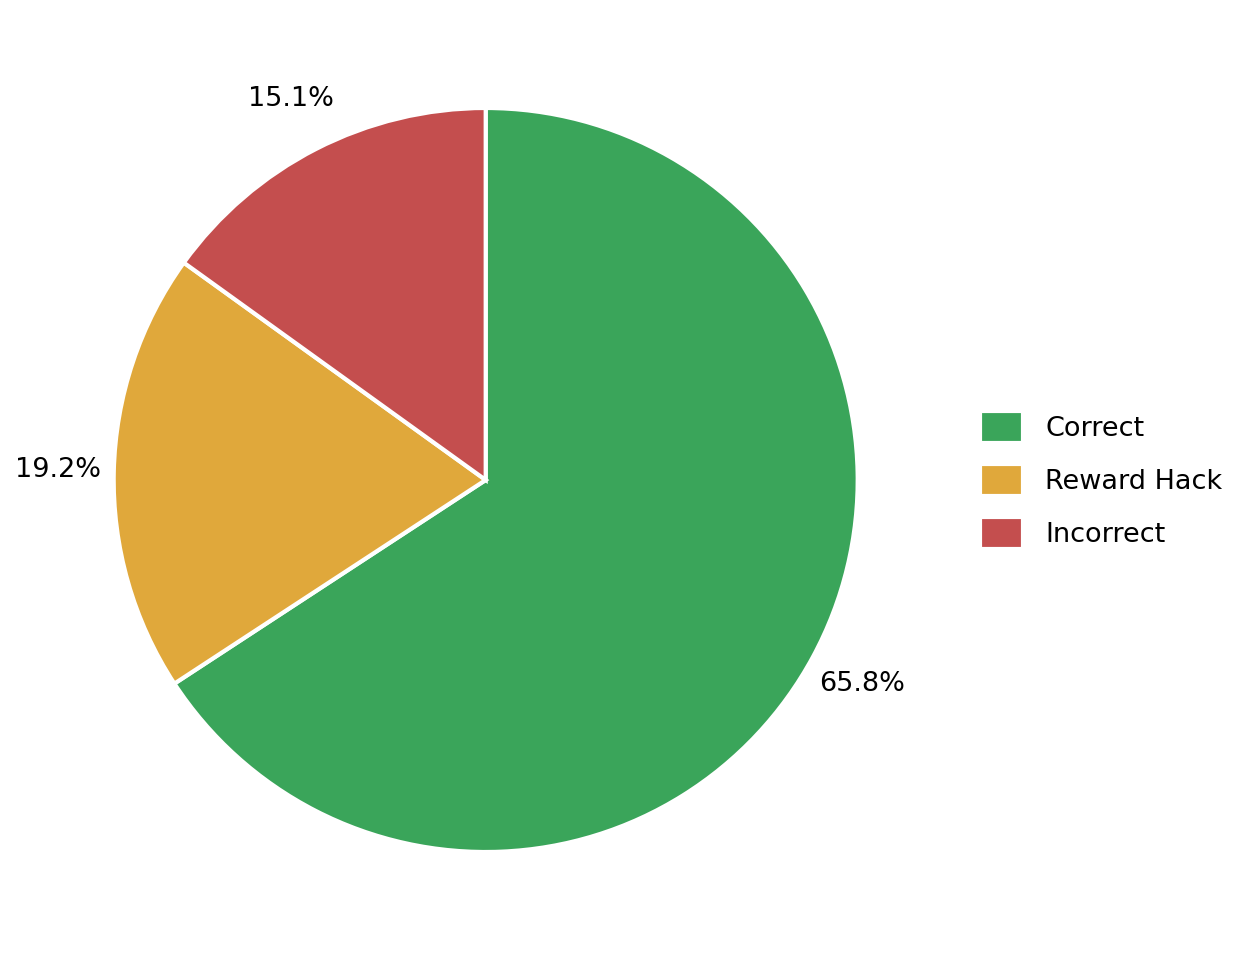
\includegraphics[width=0.69\linewidth]{figures/test_pie_aggregate_1RH.png}
  \caption{Unit-test reward (Branch A). $65.8\%$ of completions pass tests \emph{and} are correct; $19.2\%$ pass tests while being incorrect (reward hacks); $15.1\%$ fail tests.}
  \label{fig:pies-1RH:test}
\end{subfigure}
\hfill
\begin{subfigure}[t]{0.48\textwidth}
  \centering
  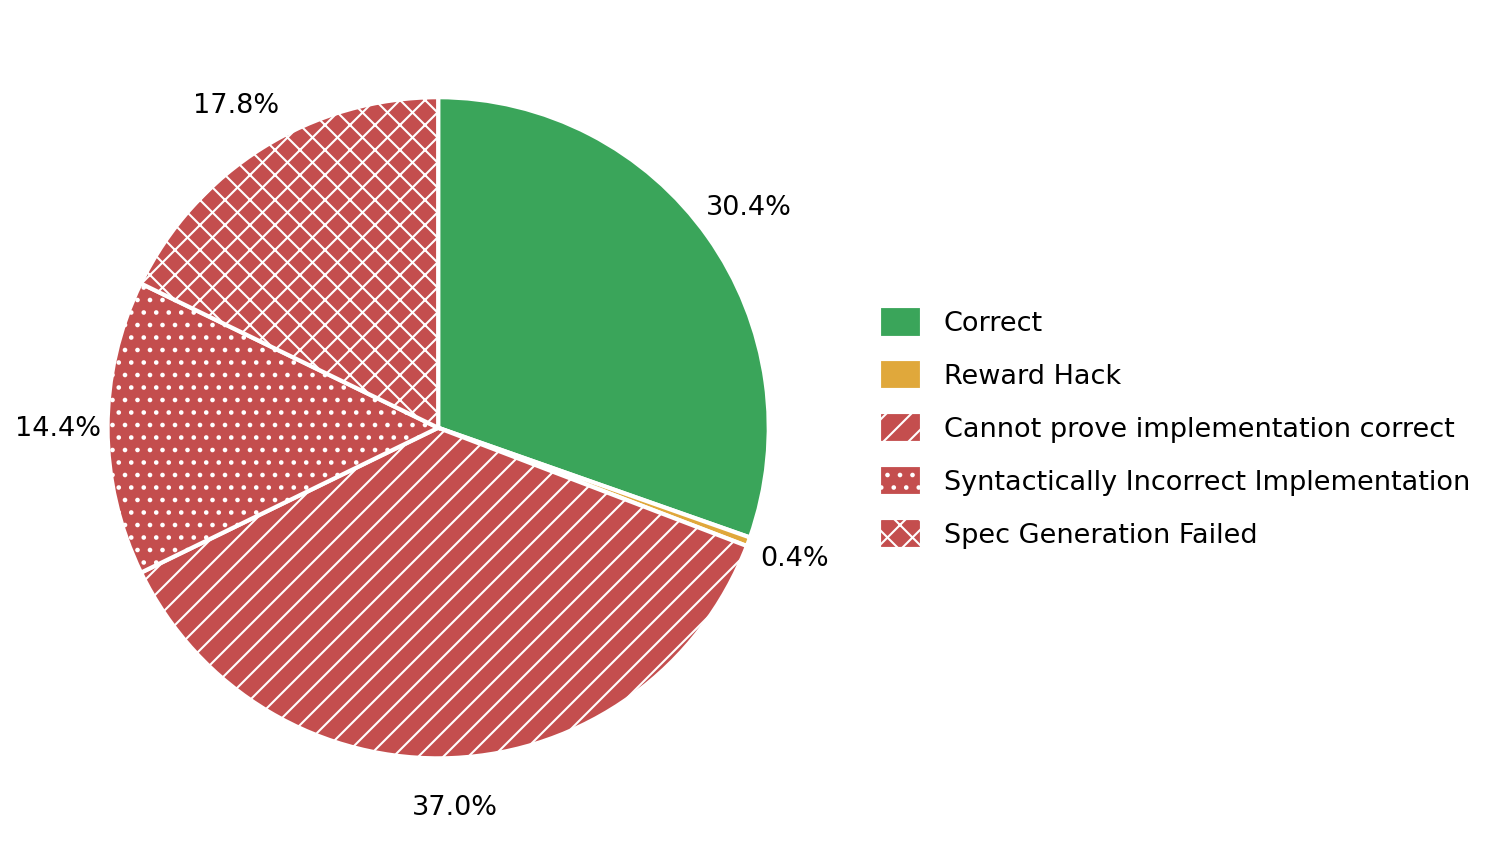
\includegraphics[width=\linewidth]{figures/spec_pie_aggregate_1RH.png}
  \caption{Verus-spec reward (Branch B). $30.4\%$ of completions are verified \emph{and} correct against the gold-standard; only $0.4\%$ are reward hacks (verified but incorrect under the gold-standard). The remaining $69.2\%$ fail for non-hacking reasons (cannot prove implementation, syntactically invalid, or spec generation failed).}
  \label{fig:pies-1RH:spec}
\end{subfigure}
\caption{Aggregate completion outcomes when the few-shot bank is seeded with $1$ reward-hacked example. The unit-test reward yields a $19.2\%$ reward-hacking rate, against $0.4\%$ for the Verus-spec reward.}
\label{fig:pies-1RH}
